\begin{usecase}{08}{Lista degli eventi del regolatore semaforico}
\usecaseprimaryactors{Utente autenticato}
\usecasepre{L'utente sta visionando il dettaglio del regolatore semaforico selezionato dalla lista.}
\usecasedesc{Viene visualizzata la lista degli eventi relativi al regolatore semaforico selezionato per la data corrente.}
\usecasepost{Viene visualizzata la lista degli eventi relativi al regolatore semaforico selezionato per la data corrente.}
\label{uc:UC08}
\end{usecase}

\begin{figure}[!h] 
    \centering 
    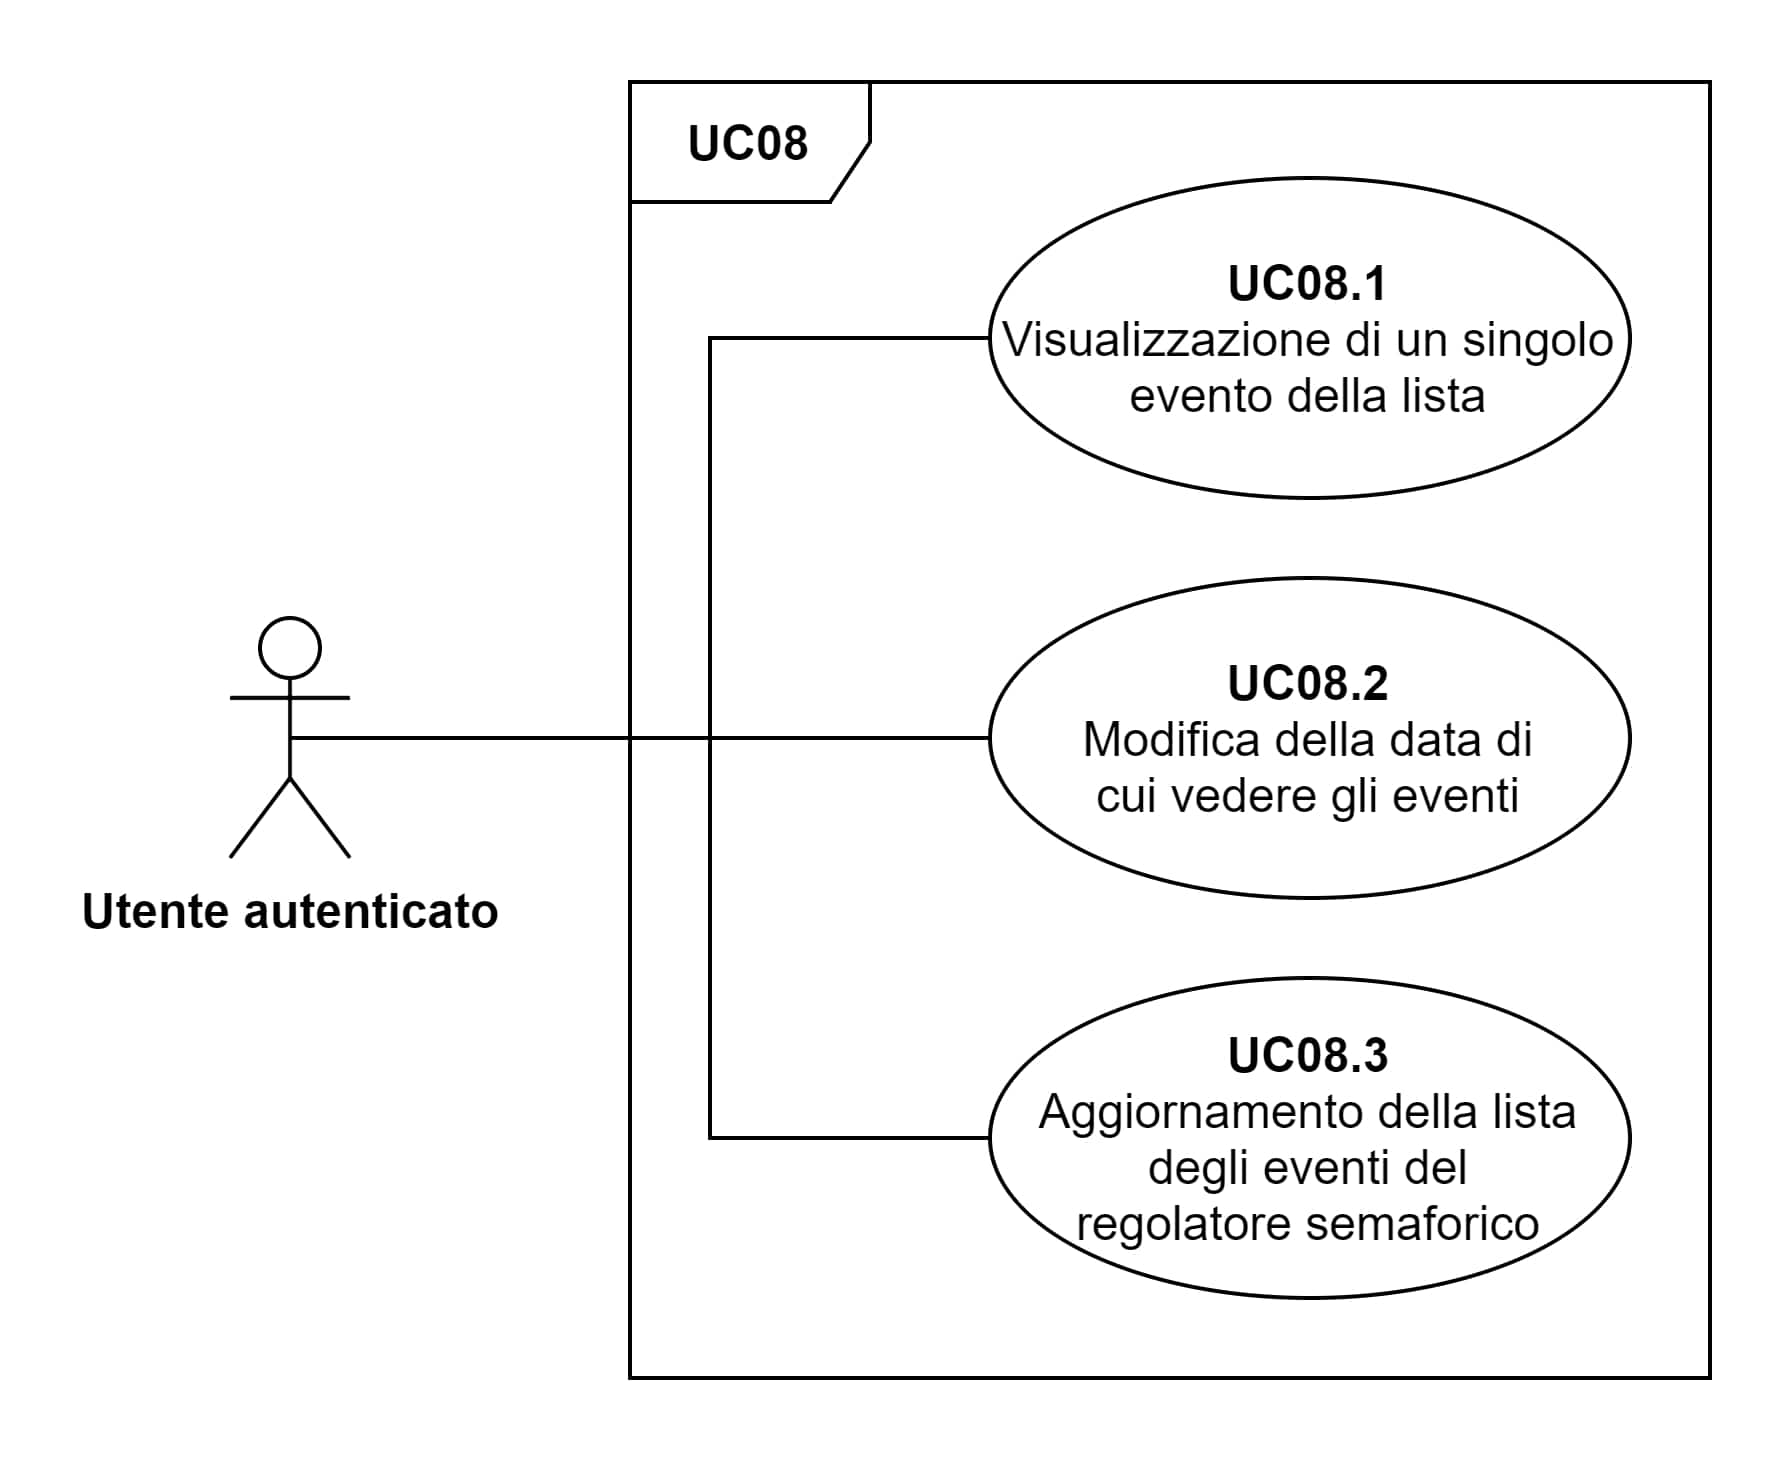
\includegraphics[width=1.0\columnwidth]{appendice-A/uc08} 
    \caption{SMacs - Sotto-casi d'uso di UC08 - Lista degli eventi del regolatore semaforico}
\end{figure}

\begin{usecase}{08.1}{Visualizzazione di un singolo evento della lista}
\usecaseprimaryactors{Utente autenticato}
\usecasepre{L'utente sta visionando la lista degli eventi del regolatore semaforico.}
\usecasedesc{Viene visualizzato un singolo evento relativo al regolatore semaforico della lista, mostrando un icona che rappresenta la gravità dell'evento e un breve messaggio descrittivo.}
\usecasepost{Viene visualizzato un singolo evento relativo al regolatore semaforico della lista, mostrando un icona che rappresenta la gravità dell'evento e un breve messaggio descrittivo.}
\label{uc:UC08-1}
\end{usecase}

\begin{usecase}{08.2}{Modifica della data di cui vedere gli eventi}
\usecaseprimaryactors{Utente autenticato}
\usecasepre{L'utente sta visionando la lista degli eventi del regolatore semaforico.}
\usecasedesc{L'utente seleziona la funzionalità di aggiornamento e aggiorna la data di visualizzazione degli eventi del regolatore semaforico.}
\usecasepost{L'utente seleziona la funzionalità di aggiornamento e aggiorna la data di visualizzazione degli eventi del regolatore semaforico.}
\label{uc:UC08-2}
\end{usecase}

\begin{usecase}{08.3}{Aggiornamento della lista degli eventi del regolatore semaforico}
\usecaseprimaryactors{Utente autenticato}
\usecasepre{L'utente sta visionando la lista degli eventi del regolatore semaforico.}
\usecasedesc{L'utente seleziona la funzionalità di aggiornamento e viene aggiornata la lista degli eventi del regolatore semaforico.}
\usecasepost{L'utente seleziona la funzionalità di aggiornamento e viene aggiornata la lista degli eventi del regolatore semaforico.}
\label{uc:UC08-3}
\end{usecase}